\documentclass[UTF8,zihao=5]{ctexart}

\usepackage[a4paper,left=2.05cm,right=1.85cm,top=1.7cm,bottom=1.7cm]{geometry}
\usepackage{amsmath,amssymb}
\usepackage{enumitem}
\usepackage{array}
\usepackage{tikz}
\usepackage{fancyhdr}
\usetikzlibrary{automata,positioning,arrows.meta}

\setlength{\parindent}{0pt}
\setlength{\parskip}{0.2em}
\setlist[enumerate]{itemsep=0.18em,topsep=0.18em,leftmargin=1.8em}
\setlist[itemize]{itemsep=0.12em,topsep=0.12em,leftmargin=1.8em}
\newcommand{\blank}{\underline{\hspace{2.2em}}}
\newcommand{\ansbox}{\hfill（\hspace{1.6em}）}
\newcommand{\circnum}[1]{\tikz[baseline=(char.base)]{\node[draw,circle,inner sep=0.15pt,minimum size=1.05em,line width=0.35pt,font=\scriptsize] (char) {#1};}}
\newcommand{\numblank}[1]{\ensuremath{\overset{\text{\circnum{#1}}}{\underline{\hspace{2.8em}}}}}
\newcommand{\examsection}[2]{\par\medskip\noindent\textbf{#1：#2}\par}
\newcommand{\examheading}[1]{\par\medskip\noindent\textbf{#1。}\par}

\pagestyle{fancy}
\fancyhf{}
\renewcommand{\headrulewidth}{0pt}
\fancyfoot[C]{第 \thepage 页（共 6 页）}

\begin{document}

\begin{center}
  {\large 清华大学 2025--2026 学年秋季学期期末考试}\\[0.4em]
  {\LARGE \bfseries 形式语言与自动机}
\end{center}

\textbf{注意事项：}
\begin{enumerate}[label=(\arabic*)]
  \item 答卷前，考生务必将自己的班级、姓名、学号填写在试卷上。
  \item 考生必须保持试卷的整洁。考试结束后，将试卷交回。
\end{enumerate}

\examsection{一、判断题}{本题共 8 小题，每小题 2 分，共 16 分。判断下列各命题的真假性，回答 T 或 F。}

\begin{enumerate}
  \item 若 $L$ 是正规语言，则 $L$ 中字符串的子字符串所构成的集合也是正规语言。\ansbox
  \item 若 $L$ 是正规语言，$L' \subseteq L$，则 $L'$ 也是正规语言。\ansbox
  \item 正规语言与上下文无关语言的交仍是正规语言。\ansbox
  \item 不存在通用算法，判断两个上下文无关文法是否等价。\ansbox
  \item 对于有二义的上下文无关文法，存在通用算法在有限时间内输出一个其有二义性的证据。\ansbox
  \item 有两个计数器的计数器机可以模拟任何非确定图灵机。\ansbox
  \item 设问题 $A$ 和 $B$ 都是 NP 问题，且 $A$ 可多项式时间归约到 $B$。若 $B$ 是 NP-完全问题，则 $A$ 也是 NP-完全问题。\ansbox
  \item 通用语言 $L_u$ 是递归语言。\ansbox
\end{enumerate}

\examsection{二、选择题}{本题共 6 小题，每小题 2 分，共 12 分。每题给出的选项中，只有一项符合题目要求。}

\begin{enumerate}[resume]
  \item $\{wcw^R \mid w\in\{0,1\}^+\}$。\ansbox
  \item $\{0^m10^n \mid m\ge n\ge 1\}$。\ansbox
  \item $\{ww^R \mid w\in\{0,1\}^+\}$。\ansbox
  \item $\{ww \mid w\in\{0,1\}^+\}$。\ansbox
\end{enumerate}

供以上 9--12 题选择的答案 A--I：
\begin{enumerate}[label=\Alph*.]
  \item 是某个有限自动机的语言，也是某个空栈接受方式的 DPDA 的语言。
  \item 是某个有限自动机的语言，但不是任何空栈接受方式的 DPDA 的语言。
  \item 既是某个终态接受方式的 DPDA 的语言，又是某个空栈接受方式的 DPDA 的语言，但不是任何有限自动机的语言。
  \item 是某个终态接受方式的 DPDA 的语言，但不是任何空栈接受方式的 DPDA 的语言，也不是任何有限自动机的语言。
  \item 是某个无二义上下文无关文法的语言，但不是任何 DPDA 的语言。
  \item 是某个 PDA 的语言，但不是任何无二义上下文无关文法的语言。
  \item 是递归语言，但不是任何 PDA 的语言。
  \item 是递归可枚举语言，但不是递归语言。
  \item 不是递归可枚举语言。
\end{enumerate}

\newpage
\begin{enumerate}[start=13]
  \item 以下哪一项超出了上下文无关文法的表达能力？\ansbox
  \begin{enumerate}[label=\Alph*.]
    \item 上下文无关语言 $L$ 与正规语言 $R$ 的差 $L-R$。
    \item 两个上下文无关语言的并。
    \item 上下文无关语言的补。
    \item 上下文无关语言上的同态映射。
  \end{enumerate}

  \item 以下哪个问题是不可判定的？\ansbox
  \begin{enumerate}[label=\Alph*.]
    \item 给定一个递归语言 $L$，判断字符串 $w$ 是否在 $L$ 中。
    \item 给定正规语言 $L_1,L_2$，判断是否有字符串 $w\in L_1$ 并且 $w\notin L_2$。
    \item 给定一个图灵机 $M$，判断是否有长度为 2026 的字符串 $w$，使得 $M$ 接受 $w$。
    \item 给定一个图灵机 $M$，判断是否存在字符串 $w$，使得 $M$ 在 2026 步以内接受 $w$ 或停机。
  \end{enumerate}
\end{enumerate}

\examheading{三、简答题}

\begin{enumerate}[start=15]
  \item （6 分）设 CFG
  \[
    G=(\{S,A,B,C\},\{a,b,c\},P,S),
  \]
  其中 $P$ 由下列产生式构成：
  \[
    S\to AB\mid \varepsilon,\qquad
    A\to aA\mid a,\qquad
    B\to b\mid A,\qquad
    C\to cc.
  \]
  \begin{enumerate}[label=(\arabic*)]
    \item 消去 $P$ 中的 $\varepsilon$-产生式得到产生式集合 $P_1$，构成 CFG $G_1$，使得 $L(G_1)=L(G)-\{\varepsilon\}$。给出 $P_1$。
    \item 消去 $P_1$ 中的 Unit 产生式得到产生式集合 $P_2$，构成 CFG $G_2$，使得 $L(G_2)=L(G_1)$。给出 $P_2$。
    \item 消去 $P_2$ 中的无用符号得到产生式集合 $P_3$，构成 CFG $G_3$，使得 $L(G_3)=L(G_2)$。给出 $P_3$。
  \end{enumerate}

  \item （4 分）乔姆斯基范式文法 $G$（$S$ 为开始符号）的产生式集合为：

  \begin{minipage}[t]{0.53\linewidth}
  \[
    S\to AB\mid SS\mid b,
  \]
  \[
    A\to BS\mid a\mid b,
  \]
  \[
    B\to AB\mid SA.
  \]
  \end{minipage}\hfill
  \begin{minipage}[t]{0.34\linewidth}
  \vspace{-1.5em}
  \begin{center}
  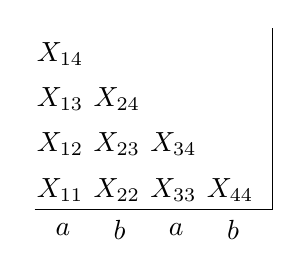
\begin{tikzpicture}[scale=0.72]
    \draw (0,0) -- (4.2,0) -- (4.2,3.2);
    \foreach \i/\x in {1/0.5,2/1.5,3/2.5,4/3.5} {
      \node at (\x,-0.35) {$\ifcase\i\or a\or b\or a\or b\fi$};
    }
    \node at (0.45,0.35) {$X_{11}$};
    \node at (1.45,0.35) {$X_{22}$};
    \node at (2.45,0.35) {$X_{33}$};
    \node at (3.45,0.35) {$X_{44}$};
    \node at (0.45,1.15) {$X_{12}$};
    \node at (1.45,1.15) {$X_{23}$};
    \node at (2.45,1.15) {$X_{34}$};
    \node at (0.45,1.95) {$X_{13}$};
    \node at (1.45,1.95) {$X_{24}$};
    \node at (0.45,2.75) {$X_{14}$};
  \end{tikzpicture}
  \end{center}
  \end{minipage}

  上图右侧表示对于文法 $G$ 和字符串 $abab$ 应用 CYK 算法时所构造的表。
  \begin{enumerate}[label=(\arabic*)]
    \item 分别计算图中所有 $X_{ij}$（$1\le i,j\le 4$）。
    \item $abab$ 有哪些子串在 $L(G)$ 中？（注意子串可以是其本身或真子串）
  \end{enumerate}

\newpage
  \item （4 分）下图刻画了 PDA
  \[
    P=(\{q,p\},\{0,1\},\{Z_0,X\},\delta,q,Z_0)
  \]
  的转移规则。请严格利用课程中介绍的从空栈接受的 PDA 到 CFG 的转换算法，定义一个与该 PDA 等价的 CFG，开始符号设为 $S$。
  \begin{center}
  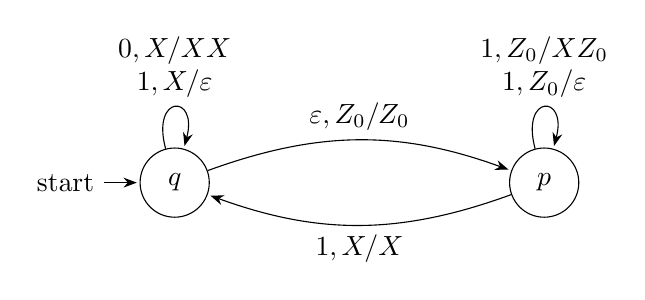
\begin{tikzpicture}[node distance=3.8cm,>=Stealth,shorten >=1pt,auto]
    \node[state,initial] (q) {$q$};
    \node[state,right=of q] (p) {$p$};
    \path[->]
      (q) edge[loop above] node[align=center] {$0,X/XX$\\$1,X/\varepsilon$} (q)
      (q) edge[bend left=20] node {$\varepsilon,Z_0/Z_0$} (p)
      (p) edge[loop above] node[align=center] {$1,Z_0/XZ_0$\\$1,Z_0/\varepsilon$} (p)
      (p) edge[bend left=20] node {$1,X/X$} (q);
  \end{tikzpicture}
  \end{center}

  \item （3 分）对于语言
  \[
    L=\{a^i b^j\mid j=i+2026\}
  \]
  可以利用 Pumping 引理证明 $L$ 不是正规语言，以下是一个证明概要：

  用反证法假设 $L$ 是正规语言，设 $n\ge 1$ 为正规语言 Pumping 引理给出的整数。
  取 $s=\numblank{1}$，则 $s\in L$。
  对任意满足条件 $s=xyz\land y\ne\varepsilon\land |xy|\le n$ 的 $x,y,z$，
  由于 $|xy|\le n$，字符串 $y$ 只可能由 $a$ 组成。取 $k=\numblank{2}$，则 $xy^kz=\numblank{3}\notin L$。

  试在其中 \circnum{1}、\circnum{2} 和 \circnum{3} 处填写适当的内容。（若需要多分支，可自行添加）

  \item （5 分）对于语言
  \[
    L=\{a^i c b^j\mid i=j^3\}
  \]
  可以利用 Pumping 引理证明 $L$ 不是上下文无关语言，以下是一个证明概要：

  用反证法假设 $L$ 是上下文无关语言，设 $n\ge 1$ 为上下文无关语言 Pumping 引理给出的整数。
  取 $z=\numblank{1}$，则 $z\in L$。
  对任意满足条件 $z=uvwxy\land vx\ne\varepsilon\land |vwx|\le n$ 的 $u,v,w,x,y$，
  如果 $c$ 在 $vx$ 中，则 $k>1$ 时 $uv^kwx^ky\notin L$；在 $c$ 不在 $vx$ 中的情况下，
  若 \numblank{2}，取 $k=\numblank{3}$，则 $uv^kwx^ky\notin L$；
  若 \numblank{4}，取 $k=\numblank{5}$，则 $uv^kwx^ky\notin L$。

  试在其中 \circnum{1}、\circnum{2}、\circnum{3}、\circnum{4} 和 \circnum{5} 处填写适当的内容。（若需要多分支，可自行添加）

  \item （5 分）可以直接使用以下两个结论：
  \begin{enumerate}[label=(\arabic*)]
    \item 若 $R$ 为正规语言，则其补 $\overline{R}$ 也是正规语言；
    \item 若 $L$ 为上下文无关语言，$R$ 为正规语言，则 $L\cap R$ 也是上下文无关语言。
  \end{enumerate}
  现有 $L$ 为上下文无关语言，$R$ 为正规语言。请仅依赖上述两个已知事实，证明 $L$ 与 $R$ 的差 $L-R$ 也是上下文无关语言。

  \item （5 分）设有两个语言 $A,B\subseteq\{0,1\}^*$，满足：
  \begin{itemize}
    \item $A$ 是递归可枚举语言，但其补 $\overline{A}$ 不是递归可枚举语言；
    \item $B$ 不是递归可枚举语言，但其补 $\overline{B}$ 是递归可枚举语言。
  \end{itemize}
  定义
  \[
    C=\{x\#y\mid x\in A\vee y\in B\},
  \]
  （此处 ``$x\#y$'' 表示由字符串 $x$、一个新符号 ``$\#$''、以及字符串 $y$ 连接得到的字符串）。分别回答并简要说明理由：
  \begin{enumerate}[label=(\arabic*)]
    \item $C$ 是否是递归可枚举语言？
    \item $\overline{C}$ 是否是递归可枚举语言？
    \item $C$ 是否是递归语言？
  \end{enumerate}
\end{enumerate}

\newpage
\examheading{四、设计题}

\begin{enumerate}[start=22]
  \item （5 分）我们知道由 CFG
  \[
    S\to (S)\mid SS\mid 0\mid \varepsilon
  \]
  定义的语言不是正规语言。但如果我们进一步限制括号嵌套的最大深度，就能得到一个正规语言，试构造接受由 CFG
  $G=(\{S_2,S_1,S_0\},\{(,),0\},P,S_2)$ 定义的语言的一个有限状态自动机（DFA、NFA 或 $\varepsilon$-NFA 均可），其中 $P$ 由下列产生式构成：
  \[
    S_2\to (S_1)\mid S_2S_2\mid 0\mid \varepsilon,
  \]
  \[
    S_1\to (S_0)\mid S_1S_1\mid 0\mid \varepsilon,
  \]
  \[
    S_0\to S_0S_0\mid 0\mid \varepsilon
  \]

  \item （5 分）试构造下列语言的一个正规表达式：
  \[
    L=\{w\in\{0,1\}^*\mid w\text{ 是某个自然数 }n\text{ 的二进制表示，其中 }n\text{ 是 }3\text{ 的倍数}\}.
  \]
  例如：$0,11\in L$，$\varepsilon,10,011\notin L$。

  \item （5 分）试构造下列语言的一个 CFG：
  \[
    L=\{a^m b^n\mid m,n\ge 0\land m\le 2n\land n\le 2m\}.
  \]

  \item （5 分）试构造以终态接受方式接受下列语言的一个 PDA（给出状态转移图）：
  \[
    L=\{a^i b^j c^k\mid i,j,k\ge 0\land i+k=j\}.
  \]

  \item （5 分）左下方的状态转移图表示一个图灵机子程序 \textit{Triple}，你可以用右下方的示意图来表示这个子程序：
  \begin{center}
  \begin{minipage}[c]{0.64\linewidth}
  \centering
  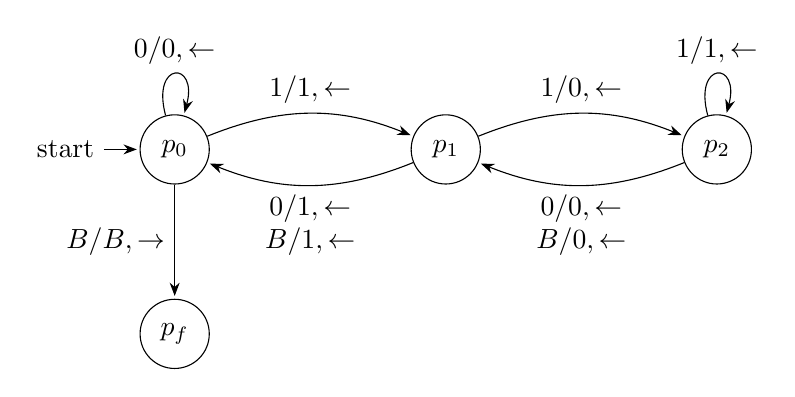
\begin{tikzpicture}[node distance=2.55cm,>=Stealth,shorten >=1pt,auto]
    \node[state,initial] (p0) {$p_0$};
    \node[state,right=of p0] (p1) {$p_1$};
    \node[state,right=of p1] (p2) {$p_2$};
    \node[state,below=1.45cm of p0] (pf) {$p_f$};
    \draw[->] (p0) edge[loop above] node {$0/0,\leftarrow$} (p0);
    \draw[->] (p2) edge[loop above] node {$1/1,\leftarrow$} (p2);
    \draw[->] (p0) -- node[left] {$B/B,\to$} (pf);

    \draw[->] (p0) to[bend left=22] node[above] {$1/1,\leftarrow$} (p1);
    \draw[->] (p1) to[bend left=22] node[below,align=center] {$0/1,\leftarrow$\\$B/1,\leftarrow$} (p0);

    \draw[->] (p1) to[bend left=22] node[above] {$1/0,\leftarrow$} (p2);
    \draw[->] (p2) to[bend left=22] node[below,align=center] {$0/0,\leftarrow$\\$B/0,\leftarrow$} (p1);
  \end{tikzpicture}
  \end{minipage}\hfill
  \begin{minipage}[c]{0.30\linewidth}
  \centering
  \fbox{\begin{minipage}{0.9\linewidth}
    \centering
    \textit{Triple}\\[0.3em]
    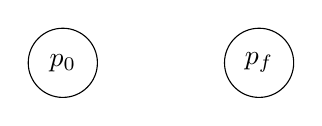
\begin{tikzpicture}[node distance=1.6cm,>=Stealth,baseline=-0.5ex]
      \node[state] (a) {$p_0$};
      \node[state,right=of a] (b) {$p_f$};
    \end{tikzpicture}
  \end{minipage}}
  \end{minipage}
  \end{center}
  试设计一个图灵机
  \[
    M=(Q,\{0,1\},\Gamma,\delta,q_0,B,F)
  \]
  接受如下语言：
  \[
  \begin{aligned}
    L=\{\,w\in L(1(0+1)^*)\mid{}&
    \text{存在正整数 }m,n,\ w\text{ 是 }n\text{ 的二进制表示，}\\
    &\text{且 }3^m n\text{ 的二进制表示不包含连续的 }3\text{ 个 }1\,\}.
  \end{aligned}
  \]
  用状态转移图描述你所设计的图灵机；如果你没有用到子程序 \textit{Triple}，请写出设计思路。
\end{enumerate}

\newpage
\examheading{五、证明题}

\begin{enumerate}[start=27]
  \item （4 分）设
  \[
    L=\{1^x2^y3^a4^b\in\Sigma^*\mid a+b\ne xy\}
  \]
  是字母表 $\Sigma=\{1,2,3,4\}$ 上的语言。试证明 $L$ 不是正规语言。

  \item （5 分）给定一个 DFA
  \[
    A=(Q,\Sigma,\delta,q_0,F),
  \]
  我们通过下列方法构造接受 $L(A)^R$ 的 $\varepsilon$-NFA $A_R$：
  \begin{enumerate}[label=(\arabic*)]
    \item 把 $A$ 的状态转移图中的所有箭弧反转；
    \item 新自动机唯一的接受状态是 $A$ 的初始状态；
    \item 创建一个新的初始状态 $p_0$，从该状态出发到所有 $A$ 的接受状态都建立一个 $\varepsilon$ 转移。
  \end{enumerate}
  记
  \[
    A_R=(Q\cup\{p_0\},\Sigma,\delta_R,p_0,\{q_0\}),
  \]
  有
  \[
    \forall w\in\Sigma^*,\ \forall q\in Q,\qquad
    \hat{\delta}(q,w)\in F \Longleftrightarrow q\in\hat{\delta}_R(p_0,w^R).
  \]
  对 $\varepsilon$-NFA $A_R$ 进行子集构造，得到 DFA $A'_R$。设 $x,y\in Q$ 是 $A$ 的两个状态，试证明：$x$ 和 $y$ 是可区分的当且仅当在一个 $A'_R$ 的可达状态 $S$ 使 $x,y$ 恰有其一在 $S$ 中。

  \item （6 分）设 $L$ 是字母表 $\Sigma$ 上的语言，令
  \[
    L'=\{w\in\Sigma^*\mid \exists \alpha,\beta\in\Sigma^*\ \text{s.t.}\ \alpha w\beta\in L\}.
  \]
  若 $L$ 是上下文无关语言，试问 $L'$ 是否一定是上下文无关语言？反之，若 $L'$ 是上下文无关语言，试问 $L$ 是否一定是上下文无关语言？证明你对于这两个问题的结论。

\end{enumerate}

\examheading{附加题，直接加入总评成绩}
\begin{enumerate}[start=30]
  \item （5 分）设 $A,B$ 为字母表 $\Sigma$ 上的语言。考虑关于语言 $X\subseteq\Sigma^*$ 的语言方程
\[
  X=AX\cup B.
\]
若 $\varepsilon\notin A$，试写出该方程的解，并证明解的唯一性。
\end{enumerate}

\newpage
\null

\end{document}
